\mysection{РАЗРАБОТКА ПРИЛОЖЕНИЯ}

\subsection{Подготовка окружения для разработки}

Как было сказано ранее, основой разрабатываемого приложения будет являться JavaScript-фреймворк Vue.js. Данный фреймворк позволяет начать работу над проектом максимально просто -- достаточно добавить на веб-страницу необходимую версию JavaScript-файла с~кодом Vue.js, используя тег \,\verb|<script>|.

Однако, для обеспечения удобства разработки и~возможности использования новейших возможностей языка JavaScript было решено использовать пакетный менеджер NPM [?] вместе с~компилятором Babel [?] и~утилитой Webpack [?] -- одним из наиболее популярных на данный момент [?] инструментом для сборки веб-приложений.


\subsubsection{Пакетный менеджер NPM}

NPM (аббр. \emph{Node Package Manager}) -- менеджер пакетов, входящий в~став программной платформы Node.js [?]. NPM существенно упрощает установку компонентов, необходимых для работы или сборки приложения.

При работе с~данным пакетным менеджером, особый интерес представляет файл \textbf{package.json}. Данный файл содержит массу информации о~разрабатываемом приложении: название, версия, описание, тип лицензии и~т.д. Но наиболее важным содержимым файла package.json являются зависимости -- список имён и~версий пакетов, требующихся для работы приложения.

% TODO Примеры содержимого package.json


\subsubsection{Babel}

Babel -- транспилер (англ. \emph{transpiler}), транслирующий код JavaScript стандартов ES2015 и~новее [?] в~код более ранних версий JavaScript.

Использование подобного инструмента позволит писать код, соответствующий последним стандартам JavaScript, не теряя при этом совместимость приложения со~старыми версиями веб-браузеров.

% TODO Пример работы Babel
% TODO Список поддерживаемых браузеров?


\subsubsection{Webpack}

Webpack -- система сборки для JavaScript-приложений, предназначенная, в первую очередь, для генерирования статических ресурсов на основе JavaScript-модулей и~их зависимостей.

Одним из основных преимуществ Webpack является его способность работать с~практически любыми типами ресурсов. Данная возможность обеспечивается дополнительно устанавливаемых \emph{загрузчиков} (англ. \emph{loaders}), которые, к~примеру, позволяют:
\begin{dashitemize}
  \item производить компиляцию JavaScript-файлов с~помощью Babel;
  \item осуществлять статический анализ кода с~помощью ESLint [?];
  \item минифицировать и обфусцировать код приложения;
  \item обрабатывать файлы с~расширением <<.vue>> (однофайловые компоненты Vue.js);
  \item производить трансляцию стилей, описанных на языке SCSS [?], в~CSS.
\end{dashitemize}

Стоит также отметить, что с~помощью Webpack можно существенно облегчить разработку ве-приложения. Благодаря специальным расширениям становится возможно запустить локальный HTTP-сервер, позволяющий просматривать и~отлаживать разрабатываемое приложение в~браузере компьютера, на котором ведётся разработка.



\subsection{Структура проекта. Артефакты сборки (?)}


\subsubsection{Структура проекта}


\subsubsection{Точка входа}


\subsubsection{Артефакты сборки}



\subsection{Глобальное хранилище данных приложения. Однонаправленный поток данных}

Vuex -- библиотека-расширение для Vue.js приложений, позволяющая создавать глобальное хранилище данных, доступное для всех модулей и Vue-компонентов, входящих в~состав проекта. Подобное хранилище необходимо не только для обмена данными между компонентами -- основной его задачей является управление состоянием представлений приложения.

Идеи, лежащие в~основе данной библиотеки, унаследованы от архитектуры Flux [?], представленная компанией Facebook. Vuex предоставляет шаблонный подход к~управлению состояниями компонентов приложения, основанный на \emph{однонаправленном потоке данных}.


\subsubsection{Однонаправленный поток данных}

Взаимный обмен данными и~событиями между моделями и~представлениями может вызвать множество трудностей при увеличении числа компонентов. Асинхронные изменения и~побочные эффекты могут существенно усложнить разработку и~отладку, а~также нарушить работу приложения.

Однонаправленный поток данных в~простейшем виде представлен на рисунке \ref{fig:simple-oneway-data-flow}.

\begin{figure}[h!]
  \centering
  \setlength{\fboxsep}{5pt}
  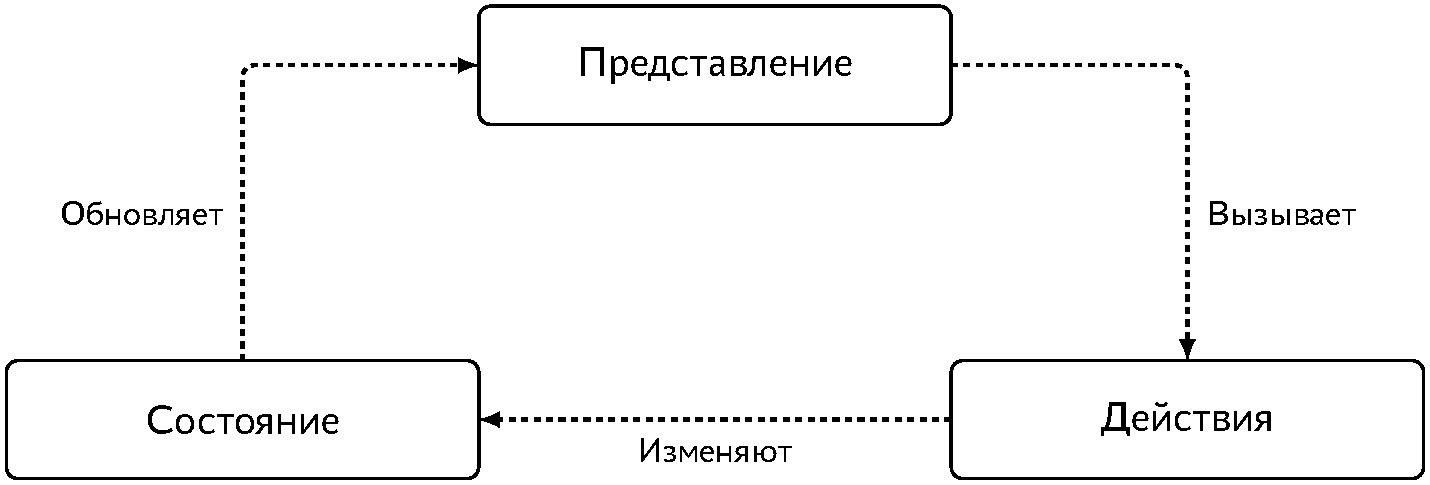
\includegraphics[width=.9\textwidth]{img/tikz/simple-oneway-data-flow/pic}
  \vspace*{12pt}
  \caption{Однонаправленный поток данных}\label{fig:simple-oneway-data-flow}
\end{figure}

Подход, описанный на рисунке \ref{fig:simple-oneway-data-flow}, прекрасно подходит для управления представлением одного компонента. Однако, при появлении нескольких компонентов, зависящих от одного и~того же состояния, структура приложения может существенно усложниться.

% TODO Сноска про <<одиночку>>?
Vuex решает проблему, описанную выше, вводя в~структуру приложения глобальное хранилище данных, являющееся состоянием-<<одиночкой>> (англ. \emph{singleton}), которое обновляет все необходимые представления с~помощью реактивных обновлений.

Для избежания неконтролируемых изменений состояния в~Vuex введено следующее ограничение: изменить состояние можно только с~помощью синхронных транзакций, называемых \emph{мутациями}.

Асинхронные операции, результаты выполнения которых изменяют состояние, в~Vuex получили название \emph{<<действия>>}. Внутри функций-обработ-чиков действий становится возможно, к~примеру, совершить асинхронный запрос к~серверу, а~при получении результата сделать одну или более синхронных мутаций состояния.

Схема организации однонаправленного потока данных при использовании Vuex изображена на рисунке \ref{fig:vuex-oneway-data-flow}.

\begin{figure}[h!]
  \centering
  \setlength{\fboxsep}{5pt}
  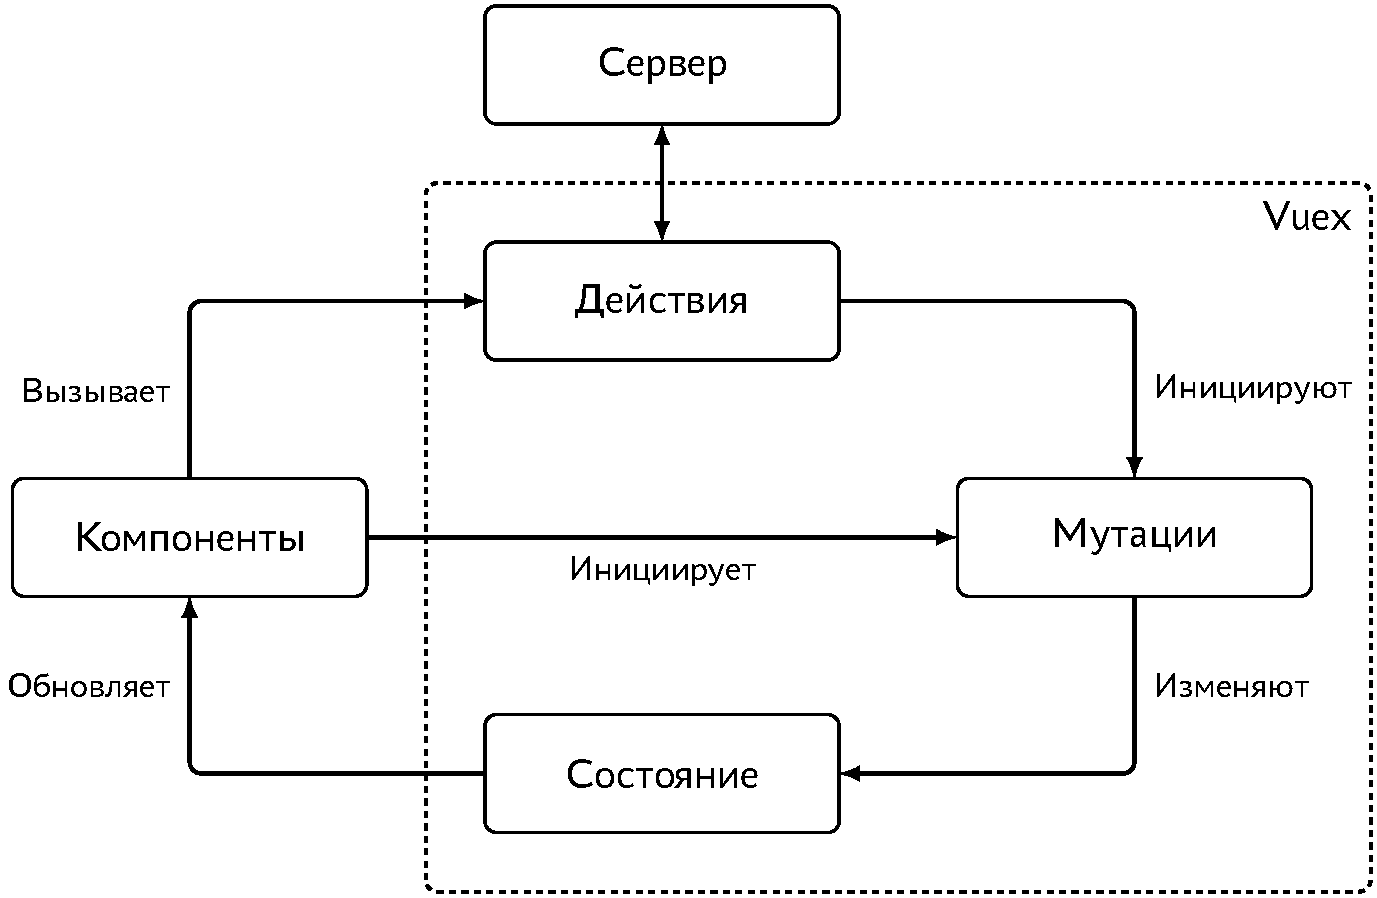
\includegraphics[width=.9\textwidth]{img/tikz/vuex-oneway-data-flow/pic}
  \vspace*{12pt}
  \caption{Однонаправленный поток данных при использовании Vuex}\label{fig:vuex-oneway-data-flow}
\end{figure}


\subsubsection{Модули хранилища данных}

Глобальные данные о состоянии приложения по умолчанию хранятся в одном и том же объекте. Рост числа модулей приложения неизбежно приводит к тому, что структура данного объекта существенно усложняется, а именование мутаций и действий может вызывать затруднения из-за требования к уникальности имён ключей.

Для решения описанных выше проблем Vuex предоставляет инструменты для разделения хранилища на \textbf{модули}. Модули представляют из себя самостоятельные части глобального состояния, каждая из которых может содержать объект с данными, мутации и т.д. При использовании данного подхода возможные проблемы с именованием мутаций и действий решаются благодаря тому, что каждый модуль Vuex может иметь собственное пространство имён.

% TODO Добавить пример работы с модулями

Хранилище Vuex, используемое в разрабатываемом приложении, было разделено на модули, соответствующие важнейшим подсистемам программного обеспечения устройств Reach и Reach~RS:
\begin{dashitemize}
  \item позиционирование и режим RTK;
  \item конфигурация устройства;
  \item входящие и исходящие потоки данных;
  \item состояние компонентов графического интерфейса.
\end{dashitemize}

Схема модулей глобального хранилища, используемого в приложении, изображена на рисунке \ref{fig:vuex-modules}.

\begin{figure}[h!]
  \centering
  \setlength{\fboxsep}{5pt}
  \includegraphics[width=.75\textwidth]{example-image}
  \vspace*{12pt}
  \caption{Модули хранилища Vuex}\label{fig:vuex-modules}
\end{figure}



\subsection{Модули и компоненты приложения}

В пунктах, следующих далее, описана структура и организация модулей и компонентов разрабатываемого веб-приложения. Первые два пункта посвящены модулям общего назначения и вспомогательным компонентам, которые необходимы для создания моделей представления, описанных в подразделе \ref{subsec:app-modules-requirements}. Сами же модели представления описаны в третьем пункте текущего подраздела.


\subsubsection{Модули общего назначения}

Как было сказано ранее, к модулям общего назначения относятся модуль работы с картами и модуль обработки событий. Рассмотрим каждый из их подробнее.

\paragraph{Модуль работы с картами}

Модуль работы с картами представляет из себя обёртку (англ. \emph{wrapper}) над частью библиотеки OpenLayers, используемой в разрабатываемом приложении для отображения карт и различной информации на них. Код модуля содержится в файле \emph{olWrapper.js}.

Данный модуль предназначен для повышения удобства создания однотипных карт -- для добавления карты на определённую страницу достаточно импортировать модуль в нужную часть кода приложения и вызвать соответствующие функции.

Импорт необходимых модулей OpenLayers, единожды осуществляемый в модуле работы с картами (см.~листинг \ref{lst:modules__maps__imports}), исключает повторение существенного количества строк кода и уменьшает размер файла vendor.js.

\lstinputlisting[
  caption={olWrapper.js: импорт необходимых модулей OpenLayers},
  label={lst:modules__maps__imports}
]{src/modules__maps__imports.js}


\paragraph{Модуль обработки событий}



\subsubsection{Вспомогательные компоненты}


\subsubsection{Модели представления}

\paragraph{Статус}

\paragraph{Модули настройки параметров устройства}

\paragraph{Модули настройки входящих и исходящих потоков данных}

\paragraph{Модули настройки беспроводных соединений}

\paragraph{Общие настройки}

\newpage
